% Command to set a chapter's name different in TOC and document
% The first {} is for the chatper's name in TOC
% The second {} is for the chapter's name in the document
% Texorpdfstring write {} as a text in the document and the second {} as bookmark
\begin{browserSubsections}
\mychaptertwo{\texorpdfstring{1er Conversatorio}{1ER CONVERSATORIO}}{1er Conversatorio\\[1cm] Experiencias que trascienden fronteras}

\newpage
{\hoffset=0pt
	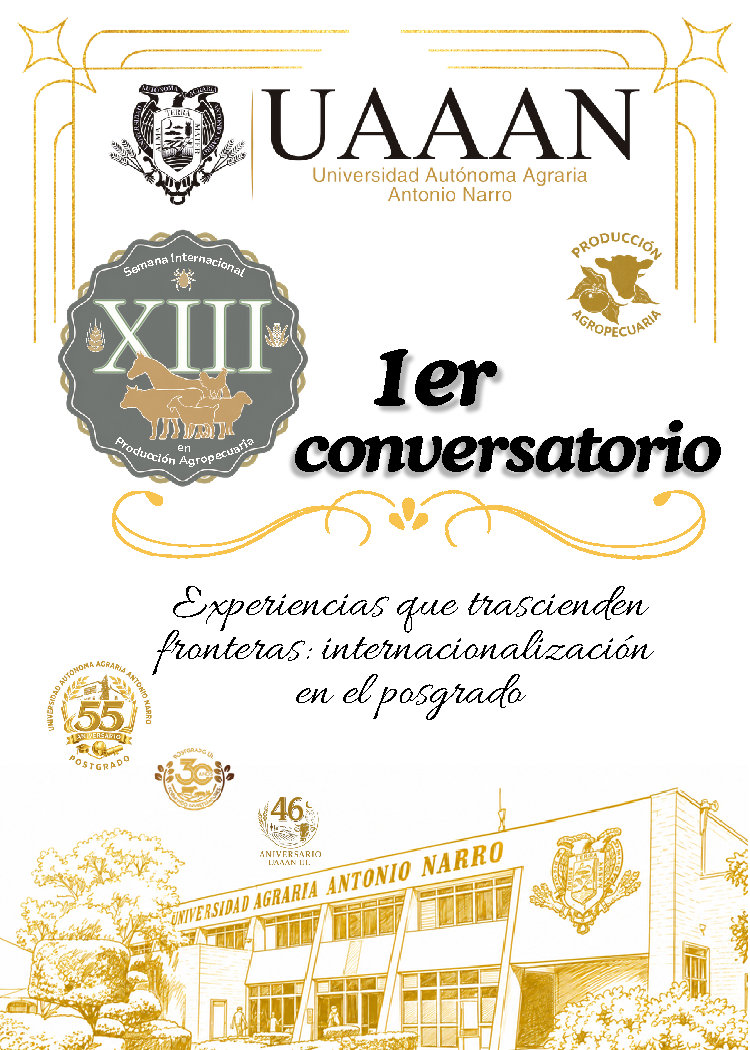
\includepdf[fitpaper=true,pages=-,width=\paperwidth, pages={1,2}]{images/events/sipa xiii discussion.pdf}
}

\newpage
% Command to add a section name, without numbering and dots line in chapter style
% The cirst line edits the indentation of the TOC text
% The second command moves the line to the left, blacknes the text and shortens the distance from the text under it
% The last command restores the indentation of the TOC text
\cftsetindents{section}{0.5cm}{2cm}
\phantomsection
\cftaddtitleline{toc}{section*}{%
	\hspace{0.49cm}\textbf{\MakeUppercase{Experiencias que trascienden fronteras: Internacionalización en el posgrado}}\vspace{-2.5mm}%
}{}
\cftsetindents{section}{1.5cm}{2cm}

\newpage
\begin{wrap}
	\chapter{introduction}
	% If you're using TexStudio, this line helps you to identify the keynote/document/course in the editor's TOC
\end{wrap}

% Adds a section name without printing it in TOC
\phantomsection
\pdfbookmark[0]{\MakeUppercase{Experiencias que trascienden fronteras: Internacionalización en el posgrado}}{}
\section*{\MakeUppercase{Experiencias que trascienden fronteras: Internacionalización en el posgrado}}

\vspace{-0.2cm}
% Name of the section in header
\nombsec{Experiencias que  trascienden: Internacionalización en el posgrado}
% This function adds the name in the TOC
\tocauthor{Ma. Guadalupe Calderón Leyva}
\author{%
	Ma. Guadalupe Calderón Leyva
}
\ijaffiliation{%
	Jefa del postgrado en Ciencias en Producción Agropecuaria
}
\corresponding{}{}
% As no title is placed in this \maketitle, the space is reduced to avoid blanc lines in TOC
\title{\vspace{-5mm}}

% Function to remove the bookmark placed by \maketitle
\begingroup
\ijauthorbookmarkfalse
\maketitle
\endgroup

Un conversatorio es un espacio de diálogo e intercambio de experiencias en el que los participantes comparten experiencias, conocimientos, opiniones y reflexiones sobre un tema en común, generalmente a partir de preguntas orientadoras y con interacción con el público. Tomando en cuenta lo anteriormente dicho, este conversatorio tiene como objetivo generar un espacio de diálogo e intercambio de experiencias sobre estancias académicas internacionales, que permita los estudiantes, tanto internos como externos, conocer de primera mano las oportunidades, aprendizajes y retos de la movilidad internacional, promoviendo una visión global y motivándolos a explorar nuevas oportunidades de formación y colaboración académica.

\begin{table}[H]
	\centering
	\begin{tabular}{cc}
		\multicolumn{2}{c}{\textbf{Schedule}} \\
		\multicolumn{1}{c|}{\multirow{1}{*}{Septiember, 11}} & 9:30 am \\
	\end{tabular}
\end{table}

% Adds the section name in toc without printing the section number
\phantomsection
\section*{PRESENTACIÓN DE AUTORIDADES}
\addcontentsline{toc}{section}{\hspace{-0.1cm}\texorpdfstring{\MakeUppercase{PRESENTACIÓN DE AUTORIDADES}}{\MakeUppercase{PRESENTACIÓN DE AUTORIDADES}}}
\vspace{1.5cm}

\begin{wrap}
	\chapter{Introduction talk}
	% If you're using TexStudio, this line helps you to identify the keynote/document/course in the editor's TOC
\end{wrap}
\cero
% Name of the section in header.
% Given that a fixed name was established for this part of the document, the function can be omited to avoid more changes
%\nombsec{}
% This function adds the name in the TOC
\tocauthor{Dr. Antonio Flores Naveda}
\author{%
	Dr. Antonio Flores Naveda
}
\ijaffiliation{%
	Subdirector de Postgrado -- Universidad Autónoma Agraria Antonio Narro
}
\corresponding{}{}
\title{Introduction talk}

\maketitle
%\vspace{1.3cm}

\newpage
\begin{wrap}
	\chapter{Presentation}
	% If you're using TexStudio, this line helps you to identify the keynote/document/course in the editor's TOC
\end{wrap}
\cero
% Name of the section in header.
% Given that a fixed name was established for this part of the document, the function can be omited to avoid more changes
%\nombsec{}
% This function adds the name in the TOC
\tocauthor{M. C. Alexis Gabriel Pivaral Chávez}
\author{%
	M. C. Alexis Gabriel Pivaral Chávez
}
\ijaffiliation{%
	Estudiante de Doctorado en Ciencias en Producción Agropecuaria
}
\corresponding{}{}
\title{Conoce el Posgrado de la UAAAN: Formación, investigación y oportunidades profesionales}

\maketitle

\vspace*{.5cm}
\begin{resumen}
	\justifying
	El Posgrado de la \textbf{Universidad Autónoma Agraria Antonio Narro (UAAAN)} constituye un espacio de formación especializada, investigación e innovación orientado a atender las necesidades y desafíos del sector agropecuario desde una perspectiva ambiental, social, científica y económica. La institución cuenta con programas de especialidad, maestría y doctorado en diversas áreas de conocimiento relacionadas con las ciencias agrarias, la producción agropecuaria, el manejo sustentable de recursos anturales y el desarrollo e innovación científica y tecnológica; que permiten a los cursantes desarrollar competencias avanzadas para la generación y aplicación de conocimiento. En particular, la \textbf{Maestría y el doctorado en Ciencias en Producción agropecuaria} tienen como propósito formar investigadors y profesionistas especializados en el estudio y atención de problemáticas relacionadas con la producción agrícola y pecuaria, así como la innovación tecnológica y el manejo sustentable de los recursos naturales. La formación de los estudiantes en el programa de \textbf{Ciencias en Producción Agropecuaria} se complementa mediante la participación en proyectos de investigación, seminarios, cursos teórico-prácticos, congresos nacionales e internacionales, y actividades de intercambio académico y científico. Entre estas actividades, destaca la \textbf{Semana Internacional en Producción Agropecuaria}, organizada por el propio programa de posgrado para funjir como un espacio de divulgración, intercambio y vinculación académica, científica y profecional, en donde se presentan los avances y capacidades desarrolladas por los estudiantes, docentes e investigadores del programa. Las principales líneas y áreas de investigación del programa de Posgrado en Ciencias en Producción Agropecuaria abarcan disciplinas relacionadas con la producción agrícola y pecuaria, fitomejoramiento, horticultura, parasitología, biotecnología, recursos naturales, producción vegetal, sanidad agrícola, y apicultura, así como reproducción, nutrición y bienestar animal. Asimismo, estos programas fomentan la vinculación y colaboración con instituciones nacionales e internacionales, ofreciendo oportunidades de movilidad académica con instituciones de América Latina y Europa, y brindando diversas alternativas de desarrollo profesional en los ámbitos académicos, científicos, productivos, empresariales y gubernamentales. En conjunto, la \textbf{Maestría y el Doctorado en Ciencias en Producción Agropecuaria} representan una oportunidad para la formación de profesionistas e investigadores capaces de generar conocimiento, desarrollar soluciones innovadoras, y participar en la atención de los desafíos actuales del sector agropecuario, contribuyendo a su desarrollo y al manejo sustentable de los recursos naturales.
\end{resumen}

\newpage
\begin{wrap}
	\chapter{Semblance}
	% If you're using TexStudio, this line helps you to identify the keynote/document/course in the editor's TOC
\end{wrap}
% Adds a section name without printing it in TOC
\phantomsection
\section*{Discussion forum's semblances}
% Adds the section name in toc without printing the section number
\addcontentsline{toc}{section}{\hspace{-0.1cm}\texorpdfstring{DISCUSSION FORUM'S SEMBLANCE}{DISCUSSION FORUM'S SEMBLANCE}}

\begin{wrap}
	\chapter{Romeo}
	% If you're using TexStudio, this line helps you to identify the keynote/document/course in the editor's TOC
\end{wrap}
% Semblance of the discussion participants
% The main difference between the semblance and the conference blocks, it's that the semblance block only allows the display of the person's own image
% There seems to be a bug only in the first block under a section. this can be solved adding additional lines and rising the space between the text and the image
% Be careful, if you dont add the \\ & \newline, the text will be raised, but the initial paragraph will stay in it's original place
%\phantomsection
%\pdfbookmark[2]{Ing. Romeo Velasco Santiago}{}
\bandera{}
\confname{Ing. Romeo Velasco Santiago}
\confsch{Estudiante de la Maestría Profesional en Tecnología de Granos y Semillas}
\confimgone{images/semblance/sipa xiii semblance 1}
\semblancetext{8}{1}{%
	\vspace{-12mm}%
	\raisebox{-4.5mm}{\\}\newline
	El Ing. Romeo Velasco Santiago, originario del estado de Chiapas, es egresado de la carrera de Ingeniero Agrónomo en Producción, en la Universidad Autónoma Agraria Antonio Narro. Su interés en la producción y mejoramiento de cultivos básicos lo llevó a cursar actualmente la Maestría Profesional en Tecnología de Granos y Semillas en la misma institución. Como parte de su especialización, realizó una estancia internacional en la \textbf{Universidad Federal de Pelotas, en Cap\~ao do Le\~ao, Brasil, Brasil}. Su trabajo actual se centra en la tecnología de semillas y el mejoramiento genético  decultivos resilientes, como girasol y sorgo, orientando sus esfuerzos hacia la seguridad alimentaria y la sostenibilidad agrícola, y cuenta con al menos un artículo publicado sobre el comportamiento agronómico de poblaciones de girasol con alto contenido oleico en el sureste de Coahuila, México.%
}

\semblance

\begin{wrap}
	\chapter{Katherin}
	% If you're using TexStudio, this line helps you to identify the keynote/document/course in the editor's TOC
\end{wrap}
\bandera{CO}
\confname{MVZ. Katherin Castañeda Moreno}
\confsch{Estudiante de la Maestría en Ciencias en Producción Agropecuaria}
\confimgone{images/semblance/sipa xiii semblance 2}
\semblancetext{7}{1}{%
	Katherin Castañeda Moreno es Técnica en Contabilización de Operaciones comerciales y Financieras, Técnica Auxiliar Clínica Veterinaria, Tecnóloga en Producción Ganadera y Médica Veterinaria y Zootecnista, egresada de la \textbf{Universidad Tecnológica de Pereira, Colombia}. Participó en grupos de investigación sobre biodiversidad y conservación, y fue beneficiaria de una peca parcial del Programa de Intercambio Académico Latinoamericano (PILA) en 2023. Ha participado en simponsios y congresos internacionales. Actualmente cursa la Maestría en Ciencias en Producción Agropecuaria en la Universidad Autónoma Agraria Antonio Narro. Sus intereses se enfocan en nutrición y producción caprina, fortaleciendo su formación científica mediante la investigación y el intercambio académico entre Colombia y México.%
}

\semblance

\begin{wrap}
	\chapter{Salomon}
	% If you're using TexStudio, this line helps you to identify the keynote/document/course in the editor's TOC
\end{wrap}
\bandera{}
\confname{Ing. Salomón Isaias Rodríguez Morales}
\confsch{Estudiante de la Maestría en Tecnologóa de Granos y Semillas}
\confimgone{images/semblance/sipa xiii semblance 3}
\semblancetext{7}{1}{%
	El Ing. Rodríguez Morales es originario de Las Rosas, Chiapas, egresado de la carrera Ingeriero Agrónomo en Producción por la Universidad Autónoma Agraria Antonio Narro en el año 2023. Actualmente cursa la Maestría en Tecnología de Granos y Semillas, donde se especializa en la producción y el mejoramietno genético de semillas, particularmente de sorgo y maíz. Su formación profesional incluye una estancia académica en la \textbf{Universidad Federal de Pelotas, en Cap\~ao do Le\~ao, Brasil}, enfocada en tecnología de semillas. Su trabajo se orienta al desarrollo agrícola del país, sustentado en la disciplina, la responsabilidad y el compromiso con la innovación en el sector agropecuario.%
}

\semblance

\newpage
\begin{wrap}
	\chapter{Steffanny}
	% If you're using TexStudio, this line helps you to identify the keynote/document/course in the editor's TOC
\end{wrap}
\bandera{}
\confname{M. C. Steffanny Sánchez Portillo}
\confsch{Estudiante del Doctorado en Ciencias en Agricultura Protegida}
\confimgone{images/semblance/sipa xiii semblance 4}
\semblancetext{7}{1}{%
	Steffanny Sánchez-Portillo es Ingeniera Agroindustrial por parte de la \textbf{Universidad Popular del Cesar, en Cesar, Colombia}; es Maestra en Ciencias en Tecnología de los Alumentos por la Universidad Autónoma de Coahuila y actualmente doctoranda en Ciencias en Agricultura Protegida en la Universidad Autónoma Agraria Antonio Narro. Es miembro activo del Grupo de investigación en Gestión, Investigación, Producción y Transformación Agroindustrial (GIPTA). Sus líneas de investigación incluyen producción agrícola, biofortificación de cultivos, desarrollo de alimentos funcionales y bioacctividad. Cuenta con once publicaciones registradas entrea rtículos en revistas indexadas y capítulos de libro, destacando trabajos sobre licopeno en cultivos, biofortificación con nanopartículas de hierro y zinc, y producción sostenible de tilapia con tecnología biofloc, lo que refleja un perfil que integra agroindustria, biotecnología y alimentación para contribuir a sistemas alimentarios más nutritivos y sostenibles.%
}

\semblance
\end{browserSubsections}
